\documentclass{standalone}
\usepackage{tikz}
\usetikzlibrary{patterns}
\usetikzlibrary{positioning}
\usetikzlibrary{patterns, positioning}
\usetikzlibrary{shapes.misc}
\usepackage[outline]{contour}
\contourlength{1.5pt} 
\usetikzlibrary{calc}
        \usepackage{relsize}
        \tikzset{fontscale/.style = {font=\relsize{#1}}}

\begin{document}
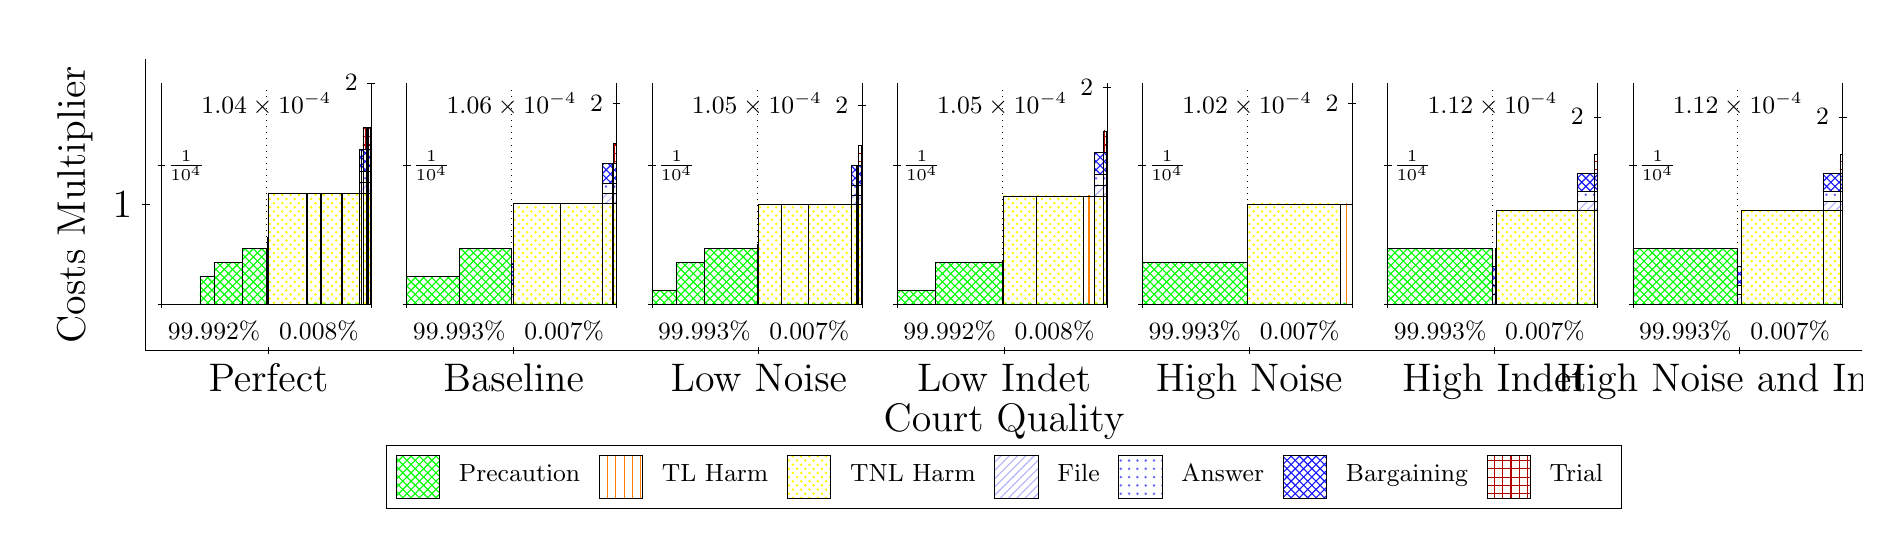
\begin{tikzpicture}
\clip(-0.5,-1.1) rectangle +(23.3,6.2);
\draw[black] (1,1) -- (1,4.7);
\node[rotate=90, fontscale=2, anchor=center] at (0.1, 2.85) {Costs Multiplier};
\draw[black] (0.95,2.85) -- (1.05,2.85);
\node[fontscale=2, anchor=east] at (0.95, 2.85) {1};

\draw[black] (1,1) -- (22.8,1);
\node[fontscale=2, anchor=center] at (11.9, 0.1) {Court Quality};
\draw[black] (2.5571,0.95) -- (2.5571,1.05);
\node[fontscale=2, anchor=north] at (2.5571, 0.95) {Perfect};
\draw[black] (5.6714,0.95) -- (5.6714,1.05);
\node[fontscale=2, anchor=north] at (5.6714, 0.95) {Baseline};
\draw[black] (8.7857,0.95) -- (8.7857,1.05);
\node[fontscale=2, anchor=north] at (8.7857, 0.95) {Low Noise};
\draw[black] (11.9,0.95) -- (11.9,1.05);
\node[fontscale=2, anchor=north] at (11.9, 0.95) {Low Indet};
\draw[black] (15.014,0.95) -- (15.014,1.05);
\node[fontscale=2, anchor=north] at (15.014, 0.95) {High Noise};
\draw[black] (18.129,0.95) -- (18.129,1.05);
\node[fontscale=2, anchor=north] at (18.129, 0.95) {High Indet};
\draw[black] (21.243,0.95) -- (21.243,1.05);
\node[fontscale=2, anchor=north] at (21.243, 0.95) {High Noise and Indet};


\draw[pattern=crosshatch, pattern color=green,draw=black,very thin] (1.6864,1.592) rectangle (1.8661,1.943);
\draw[pattern=crosshatch, pattern color=green,draw=black,very thin] (1.8661,1.592) rectangle (2.2257,2.1185);
\draw[pattern=crosshatch, pattern color=green,draw=black,very thin] (2.2257,1.592) rectangle (2.5321,2.294);
\draw[pattern=north east lines, pattern color=blue!30,draw=black,very thin] (2.5321,1.592) rectangle (2.5366,1.7324);
\draw[pattern=dots,  pattern color=blue!60,draw=black,very thin] (2.5321,1.7324) rectangle (2.5366,1.8728);
\draw[pattern=crosshatch,      pattern color=blue!90,draw=black,very thin] (2.5321,1.8728) rectangle (2.5366,2.1536);
\draw[pattern=north east lines, pattern color=blue!30,draw=black,very thin] (2.5366,1.592) rectangle (2.5427,1.7324);
\draw[pattern=dots,  pattern color=blue!60,draw=black,very thin] (2.5366,1.7324) rectangle (2.5427,1.8728);
\draw[pattern=crosshatch,      pattern color=blue!90,draw=black,very thin] (2.5366,1.8728) rectangle (2.5427,2.1536);
\draw[pattern=grid,            pattern color=red!70!black,draw=black,very thin] (2.5366,2.1536) rectangle (2.5427,2.4344);
\draw[pattern=crosshatch, pattern color=green,draw=black,very thin] (2.5427,1.592) rectangle (2.5437,1.592);
\draw[pattern=north east lines, pattern color=blue!30,draw=black,very thin] (2.5427,1.592) rectangle (2.5437,1.7324);
\draw[pattern=dots,  pattern color=blue!60,draw=black,very thin] (2.5427,1.7324) rectangle (2.5437,1.8728);
\draw[pattern=crosshatch,      pattern color=blue!90,draw=black,very thin] (2.5427,1.8728) rectangle (2.5437,2.1536);
\draw[pattern=grid,            pattern color=red!70!black,draw=black,very thin] (2.5427,2.1536) rectangle (2.5437,2.4344);
\draw[pattern=crosshatch, pattern color=green,draw=black,very thin] (2.5437,1.592) rectangle (2.5496,1.592);
\draw[pattern=north east lines, pattern color=blue!30,draw=black,very thin] (2.5437,1.592) rectangle (2.5496,1.7324);
\draw[pattern=dots,  pattern color=blue!60,draw=black,very thin] (2.5437,1.7324) rectangle (2.5496,1.8728);
\draw[pattern=crosshatch,      pattern color=blue!90,draw=black,very thin] (2.5437,1.8728) rectangle (2.5496,2.1536);
\draw[pattern=grid,            pattern color=red!70!black,draw=black,very thin] (2.5437,2.1536) rectangle (2.5496,2.4344);
\draw[pattern=crosshatch dots, pattern color=yellow,draw=black,very thin] (2.5496,1.592) rectangle (3.0354,2.996);
\draw[pattern=vertical lines, pattern color=orange,draw=black,very thin] (3.0354,1.592) rectangle (3.0519,2.996);
\draw[pattern=crosshatch, pattern color=green,draw=black,very thin] (3.0519,1.592) rectangle (3.2191,1.592);
\draw[pattern=crosshatch dots, pattern color=yellow,draw=black,very thin] (3.0519,1.592) rectangle (3.2191,2.996);
\draw[pattern=crosshatch, pattern color=green,draw=black,very thin] (3.2191,1.592) rectangle (3.2273,1.592);
\draw[pattern=vertical lines, pattern color=orange,draw=black,very thin] (3.2191,1.592) rectangle (3.2273,2.996);
\draw[pattern=crosshatch, pattern color=green,draw=black,very thin] (3.2273,1.592) rectangle (3.4803,1.592);
\draw[pattern=crosshatch dots, pattern color=yellow,draw=black,very thin] (3.2273,1.592) rectangle (3.4803,2.996);
\draw[pattern=crosshatch, pattern color=green,draw=black,very thin] (3.4803,1.592) rectangle (3.5003,1.592);
\draw[pattern=vertical lines, pattern color=orange,draw=black,very thin] (3.4803,1.592) rectangle (3.5003,2.996);
\draw[pattern=crosshatch, pattern color=green,draw=black,very thin] (3.5003,1.592) rectangle (3.7131,1.5921);
\draw[pattern=crosshatch dots, pattern color=yellow,draw=black,very thin] (3.5003,1.5921) rectangle (3.7131,2.996);
\draw[pattern=crosshatch dots, pattern color=yellow,draw=black,very thin] (3.7131,1.592) rectangle (3.7406,2.996);
\draw[pattern=north east lines, pattern color=blue!30,draw=black,very thin] (3.7131,2.996) rectangle (3.7406,3.1364);
\draw[pattern=dots,  pattern color=blue!60,draw=black,very thin] (3.7131,3.1364) rectangle (3.7406,3.2768);
\draw[pattern=crosshatch,      pattern color=blue!90,draw=black,very thin] (3.7131,3.2768) rectangle (3.7406,3.5576);
\draw[pattern=vertical lines, pattern color=orange,draw=black,very thin] (3.7406,1.592) rectangle (3.7578,2.996);
\draw[pattern=north east lines, pattern color=blue!30,draw=black,very thin] (3.7406,2.996) rectangle (3.7578,3.1364);
\draw[pattern=dots,  pattern color=blue!60,draw=black,very thin] (3.7406,3.1364) rectangle (3.7578,3.2768);
\draw[pattern=crosshatch,      pattern color=blue!90,draw=black,very thin] (3.7406,3.2768) rectangle (3.7578,3.5576);
\draw[pattern=crosshatch dots, pattern color=yellow,draw=black,very thin] (3.7578,1.592) rectangle (3.7987,2.996);
\draw[pattern=north east lines, pattern color=blue!30,draw=black,very thin] (3.7578,2.996) rectangle (3.7987,3.1364);
\draw[pattern=dots,  pattern color=blue!60,draw=black,very thin] (3.7578,3.1364) rectangle (3.7987,3.2768);
\draw[pattern=crosshatch,      pattern color=blue!90,draw=black,very thin] (3.7578,3.2768) rectangle (3.7987,3.5576);
\draw[pattern=grid,            pattern color=red!70!black,draw=black,very thin] (3.7578,3.5576) rectangle (3.7987,3.8384);
\draw[pattern=vertical lines, pattern color=orange,draw=black,very thin] (3.7987,1.592) rectangle (3.8188,2.996);
\draw[pattern=north east lines, pattern color=blue!30,draw=black,very thin] (3.7987,2.996) rectangle (3.8188,3.1364);
\draw[pattern=dots,  pattern color=blue!60,draw=black,very thin] (3.7987,3.1364) rectangle (3.8188,3.2768);
\draw[pattern=crosshatch,      pattern color=blue!90,draw=black,very thin] (3.7987,3.2768) rectangle (3.8188,3.5576);
\draw[pattern=grid,            pattern color=red!70!black,draw=black,very thin] (3.7987,3.5576) rectangle (3.8188,3.8384);
\draw[pattern=crosshatch, pattern color=green,draw=black,very thin] (3.8188,1.592) rectangle (3.8234,1.592);
\draw[pattern=crosshatch dots, pattern color=yellow,draw=black,very thin] (3.8188,1.592) rectangle (3.8234,2.996);
\draw[pattern=north east lines, pattern color=blue!30,draw=black,very thin] (3.8188,2.996) rectangle (3.8234,3.1364);
\draw[pattern=dots,  pattern color=blue!60,draw=black,very thin] (3.8188,3.1364) rectangle (3.8234,3.2768);
\draw[pattern=crosshatch,      pattern color=blue!90,draw=black,very thin] (3.8188,3.2768) rectangle (3.8234,3.5576);
\draw[pattern=grid,            pattern color=red!70!black,draw=black,very thin] (3.8188,3.5576) rectangle (3.8234,3.8384);
\draw[pattern=crosshatch, pattern color=green,draw=black,very thin] (3.8234,1.592) rectangle (3.8266,1.592);
\draw[pattern=vertical lines, pattern color=orange,draw=black,very thin] (3.8234,1.592) rectangle (3.8266,2.996);
\draw[pattern=north east lines, pattern color=blue!30,draw=black,very thin] (3.8234,2.996) rectangle (3.8266,3.1364);
\draw[pattern=dots,  pattern color=blue!60,draw=black,very thin] (3.8234,3.1364) rectangle (3.8266,3.2768);
\draw[pattern=crosshatch,      pattern color=blue!90,draw=black,very thin] (3.8234,3.2768) rectangle (3.8266,3.5576);
\draw[pattern=grid,            pattern color=red!70!black,draw=black,very thin] (3.8234,3.5576) rectangle (3.8266,3.8384);
\draw[pattern=crosshatch, pattern color=green,draw=black,very thin] (3.8266,1.592) rectangle (3.8512,1.592);
\draw[pattern=crosshatch dots, pattern color=yellow,draw=black,very thin] (3.8266,1.592) rectangle (3.8512,2.996);
\draw[pattern=north east lines, pattern color=blue!30,draw=black,very thin] (3.8266,2.996) rectangle (3.8512,3.1364);
\draw[pattern=dots,  pattern color=blue!60,draw=black,very thin] (3.8266,3.1364) rectangle (3.8512,3.2768);
\draw[pattern=crosshatch,      pattern color=blue!90,draw=black,very thin] (3.8266,3.2768) rectangle (3.8512,3.5576);
\draw[pattern=grid,            pattern color=red!70!black,draw=black,very thin] (3.8266,3.5576) rectangle (3.8512,3.8384);
\draw[pattern=crosshatch, pattern color=green,draw=black,very thin] (3.8512,1.592) rectangle (3.8643,1.592);
\draw[pattern=vertical lines, pattern color=orange,draw=black,very thin] (3.8512,1.592) rectangle (3.8643,2.996);
\draw[pattern=north east lines, pattern color=blue!30,draw=black,very thin] (3.8512,2.996) rectangle (3.8643,3.1364);
\draw[pattern=dots,  pattern color=blue!60,draw=black,very thin] (3.8512,3.1364) rectangle (3.8643,3.2768);
\draw[pattern=crosshatch,      pattern color=blue!90,draw=black,very thin] (3.8512,3.2768) rectangle (3.8643,3.5576);
\draw[pattern=grid,            pattern color=red!70!black,draw=black,very thin] (3.8512,3.5576) rectangle (3.8643,3.8384);
\node[font=\small,text=black,anchor=north] at (2.5321, 4.4) {$1.04\times 10^{-4}$};
\draw[black,very thin] (1.2,1.592) -- (1.2,4.4);
\draw[black,very thin] (1.15,1.592) -- (1.25,1.592);
\node[font=\small,text=black, anchor=west] at (1.15, 1.592) {};
\draw[black,very thin] (1.15,3.3471) -- (1.25,3.3471);
\node[font=\small,text=black, anchor=west] at (1.15, 3.3471) {$\frac{1}{10^{4}}$};

\draw[black,dotted,very thin] (2.5321,1.6762) -- (2.5321,4.3158);
\draw[black,very thin] (3.8643,1.592) -- (3.8643,4.4);
\draw[black,very thin] (3.8143,4.3999) -- (3.9143,4.3999);
\node[font=\small,text=black, anchor=east] at (3.8143, 4.3999) {\contour{white}{2}};

\draw[black,very thin] (1.2,1.592) -- (3.8643,1.592);
\draw[black,very thin] (1.2,1.542) -- (1.2,1.642);
\node[font=\small,text=black, anchor=north] at (1.2, 1.542) {};
\draw[black,very thin] (3.8643,1.542) -- (3.8643,1.642);
\node[font=\small,text=black, anchor=north] at (3.8643, 1.542) {};

\node[font=\small,text=black,anchor=south] at (1.8661, 0.992) {99.992\%};
\node[font=\small,text=black,anchor=south] at (3.1982, 0.992) {0.008\%};

\draw[pattern=crosshatch, pattern color=green,draw=black,very thin] (4.3143,1.592) rectangle (4.9803,1.943);
\draw[pattern=crosshatch, pattern color=green,draw=black,very thin] (4.9803,1.592) rectangle (5.6464,2.2941);
\draw[pattern=crosshatch, pattern color=green,draw=black,very thin] (5.6464,1.592) rectangle (5.663,1.592);
\draw[pattern=north east lines, pattern color=blue!30,draw=black,very thin] (5.6464,1.592) rectangle (5.663,1.7193);
\draw[pattern=dots,  pattern color=blue!60,draw=black,very thin] (5.6464,1.7193) rectangle (5.663,1.8466);
\draw[pattern=crosshatch,      pattern color=blue!90,draw=black,very thin] (5.6464,1.8466) rectangle (5.663,2.1013);
\draw[pattern=crosshatch, pattern color=green,draw=black,very thin] (5.663,1.592) rectangle (5.6683,1.592);
\draw[pattern=north east lines, pattern color=blue!30,draw=black,very thin] (5.663,1.592) rectangle (5.6683,1.7193);
\draw[pattern=dots,  pattern color=blue!60,draw=black,very thin] (5.663,1.7193) rectangle (5.6683,1.8466);
\draw[pattern=crosshatch,      pattern color=blue!90,draw=black,very thin] (5.663,1.8466) rectangle (5.6683,2.1013);
\draw[pattern=grid,            pattern color=red!70!black,draw=black,very thin] (5.663,2.1013) rectangle (5.6683,2.3559);
\draw[pattern=crosshatch, pattern color=green,draw=black,very thin] (5.6683,1.592) rectangle (6.2647,1.592);
\draw[pattern=crosshatch dots, pattern color=yellow,draw=black,very thin] (5.6683,1.592) rectangle (6.2647,2.8651);
\draw[pattern=crosshatch, pattern color=green,draw=black,very thin] (6.2647,1.592) rectangle (6.2652,1.592);
\draw[pattern=vertical lines, pattern color=orange,draw=black,very thin] (6.2647,1.592) rectangle (6.2652,2.8651);
\draw[pattern=crosshatch, pattern color=green,draw=black,very thin] (6.2652,1.592) rectangle (6.8031,1.5921);
\draw[pattern=crosshatch dots, pattern color=yellow,draw=black,very thin] (6.2652,1.5921) rectangle (6.8031,2.8651);
\draw[pattern=crosshatch, pattern color=green,draw=black,very thin] (6.8031,1.592) rectangle (6.9204,1.592);
\draw[pattern=crosshatch dots, pattern color=yellow,draw=black,very thin] (6.8031,1.592) rectangle (6.9204,2.8651);
\draw[pattern=north east lines, pattern color=blue!30,draw=black,very thin] (6.8031,2.8651) rectangle (6.9204,2.9924);
\draw[pattern=dots,  pattern color=blue!60,draw=black,very thin] (6.8031,2.9924) rectangle (6.9204,3.1197);
\draw[pattern=crosshatch,      pattern color=blue!90,draw=black,very thin] (6.8031,3.1197) rectangle (6.9204,3.3743);
\draw[pattern=crosshatch, pattern color=green,draw=black,very thin] (6.9204,1.592) rectangle (6.9347,1.592);
\draw[pattern=vertical lines, pattern color=orange,draw=black,very thin] (6.9204,1.592) rectangle (6.9347,2.8651);
\draw[pattern=north east lines, pattern color=blue!30,draw=black,very thin] (6.9204,2.8651) rectangle (6.9347,2.9924);
\draw[pattern=dots,  pattern color=blue!60,draw=black,very thin] (6.9204,2.9924) rectangle (6.9347,3.1197);
\draw[pattern=crosshatch,      pattern color=blue!90,draw=black,very thin] (6.9204,3.1197) rectangle (6.9347,3.3743);
\draw[pattern=crosshatch, pattern color=green,draw=black,very thin] (6.9347,1.592) rectangle (6.9782,1.592);
\draw[pattern=crosshatch dots, pattern color=yellow,draw=black,very thin] (6.9347,1.592) rectangle (6.9782,2.8651);
\draw[pattern=north east lines, pattern color=blue!30,draw=black,very thin] (6.9347,2.8651) rectangle (6.9782,2.9924);
\draw[pattern=dots,  pattern color=blue!60,draw=black,very thin] (6.9347,2.9924) rectangle (6.9782,3.1197);
\draw[pattern=crosshatch,      pattern color=blue!90,draw=black,very thin] (6.9347,3.1197) rectangle (6.9782,3.3743);
\draw[pattern=grid,            pattern color=red!70!black,draw=black,very thin] (6.9347,3.3743) rectangle (6.9782,3.629);
\draw[pattern=crosshatch, pattern color=green,draw=black,very thin] (6.9782,1.592) rectangle (6.9786,1.592);
\draw[pattern=vertical lines, pattern color=orange,draw=black,very thin] (6.9782,1.592) rectangle (6.9786,2.8651);
\draw[pattern=north east lines, pattern color=blue!30,draw=black,very thin] (6.9782,2.8651) rectangle (6.9786,2.9924);
\draw[pattern=dots,  pattern color=blue!60,draw=black,very thin] (6.9782,2.9924) rectangle (6.9786,3.1197);
\draw[pattern=crosshatch,      pattern color=blue!90,draw=black,very thin] (6.9782,3.1197) rectangle (6.9786,3.3743);
\draw[pattern=grid,            pattern color=red!70!black,draw=black,very thin] (6.9782,3.3743) rectangle (6.9786,3.629);
\node[font=\small,text=black,anchor=north] at (5.6464, 4.4) {$1.06\times 10^{-4}$};
\draw[black,very thin] (4.3143,1.592) -- (4.3143,4.4);
\draw[black,very thin] (4.2643,1.592) -- (4.3643,1.592);
\node[font=\small,text=black, anchor=west] at (4.2643, 1.592) {};
\draw[black,very thin] (4.2643,3.3471) -- (4.3643,3.3471);
\node[font=\small,text=black, anchor=west] at (4.2643, 3.3471) {$\frac{1}{10^{4}}$};

\draw[black,dotted,very thin] (5.6464,1.6762) -- (5.6464,4.3158);
\draw[black,very thin] (6.9786,1.592) -- (6.9786,4.4);
\draw[black,very thin] (6.9286,4.1382) -- (7.0286,4.1382);
\node[font=\small,text=black, anchor=east] at (6.9286, 4.1382) {\contour{white}{2}};

\draw[black,very thin] (4.3143,1.592) -- (6.9786,1.592);
\draw[black,very thin] (4.3143,1.542) -- (4.3143,1.642);
\node[font=\small,text=black, anchor=north] at (4.3143, 1.542) {};
\draw[black,very thin] (6.9786,1.542) -- (6.9786,1.642);
\node[font=\small,text=black, anchor=north] at (6.9786, 1.542) {};

\node[font=\small,text=black,anchor=south] at (4.9804, 0.992) {99.993\%};
\node[font=\small,text=black,anchor=south] at (6.3125, 0.992) {0.007\%};

\draw[pattern=crosshatch, pattern color=green,draw=black,very thin] (7.4286,1.592) rectangle (7.735,1.7675);
\draw[pattern=crosshatch, pattern color=green,draw=black,very thin] (7.735,1.592) rectangle (8.0946,2.1185);
\draw[pattern=crosshatch, pattern color=green,draw=black,very thin] (8.0946,1.592) rectangle (8.7607,2.2941);
\draw[pattern=crosshatch, pattern color=green,draw=black,very thin] (8.7607,1.592) rectangle (8.7677,1.592);
\draw[pattern=north east lines, pattern color=blue!30,draw=black,very thin] (8.7607,1.592) rectangle (8.7677,1.718);
\draw[pattern=dots,  pattern color=blue!60,draw=black,very thin] (8.7607,1.718) rectangle (8.7677,1.844);
\draw[pattern=crosshatch,      pattern color=blue!90,draw=black,very thin] (8.7607,1.844) rectangle (8.7677,2.0959);
\draw[pattern=crosshatch, pattern color=green,draw=black,very thin] (8.7677,1.592) rectangle (8.7708,1.592);
\draw[pattern=north east lines, pattern color=blue!30,draw=black,very thin] (8.7677,1.592) rectangle (8.7708,1.718);
\draw[pattern=dots,  pattern color=blue!60,draw=black,very thin] (8.7677,1.718) rectangle (8.7708,1.844);
\draw[pattern=crosshatch,      pattern color=blue!90,draw=black,very thin] (8.7677,1.844) rectangle (8.7708,2.0959);
\draw[pattern=crosshatch, pattern color=green,draw=black,very thin] (8.7708,1.592) rectangle (8.7752,1.592);
\draw[pattern=north east lines, pattern color=blue!30,draw=black,very thin] (8.7708,1.592) rectangle (8.7752,1.718);
\draw[pattern=dots,  pattern color=blue!60,draw=black,very thin] (8.7708,1.718) rectangle (8.7752,1.844);
\draw[pattern=crosshatch,      pattern color=blue!90,draw=black,very thin] (8.7708,1.844) rectangle (8.7752,2.0959);
\draw[pattern=grid,            pattern color=red!70!black,draw=black,very thin] (8.7708,2.0959) rectangle (8.7752,2.3478);
\draw[pattern=crosshatch, pattern color=green,draw=black,very thin] (8.7752,1.592) rectangle (8.7766,1.592);
\draw[pattern=north east lines, pattern color=blue!30,draw=black,very thin] (8.7752,1.592) rectangle (8.7766,1.718);
\draw[pattern=dots,  pattern color=blue!60,draw=black,very thin] (8.7752,1.718) rectangle (8.7766,1.844);
\draw[pattern=crosshatch,      pattern color=blue!90,draw=black,very thin] (8.7752,1.844) rectangle (8.7766,2.0959);
\draw[pattern=grid,            pattern color=red!70!black,draw=black,very thin] (8.7752,2.0959) rectangle (8.7766,2.3479);
\draw[pattern=crosshatch, pattern color=green,draw=black,very thin] (8.7766,1.592) rectangle (9.0685,1.592);
\draw[pattern=crosshatch dots, pattern color=yellow,draw=black,very thin] (8.7766,1.592) rectangle (9.0685,2.8517);
\draw[pattern=crosshatch, pattern color=green,draw=black,very thin] (9.0685,1.592) rectangle (9.4147,1.592);
\draw[pattern=crosshatch dots, pattern color=yellow,draw=black,very thin] (9.0685,1.592) rectangle (9.4147,2.8517);
\draw[pattern=crosshatch, pattern color=green,draw=black,very thin] (9.4147,1.592) rectangle (9.415,1.592);
\draw[pattern=vertical lines, pattern color=orange,draw=black,very thin] (9.4147,1.592) rectangle (9.415,2.8517);
\draw[pattern=crosshatch, pattern color=green,draw=black,very thin] (9.415,1.592) rectangle (9.9583,1.5921);
\draw[pattern=crosshatch dots, pattern color=yellow,draw=black,very thin] (9.415,1.5921) rectangle (9.9583,2.8518);
\draw[pattern=crosshatch, pattern color=green,draw=black,very thin] (9.9583,1.592) rectangle (10.021,1.592);
\draw[pattern=crosshatch dots, pattern color=yellow,draw=black,very thin] (9.9583,1.592) rectangle (10.021,2.8517);
\draw[pattern=north east lines, pattern color=blue!30,draw=black,very thin] (9.9583,2.8517) rectangle (10.021,2.9777);
\draw[pattern=dots,  pattern color=blue!60,draw=black,very thin] (9.9583,2.9777) rectangle (10.021,3.1037);
\draw[pattern=crosshatch,      pattern color=blue!90,draw=black,very thin] (9.9583,3.1037) rectangle (10.021,3.3556);
\draw[pattern=crosshatch, pattern color=green,draw=black,very thin] (10.021,1.592) rectangle (10.022,1.592);
\draw[pattern=vertical lines, pattern color=orange,draw=black,very thin] (10.021,1.592) rectangle (10.022,2.8517);
\draw[pattern=north east lines, pattern color=blue!30,draw=black,very thin] (10.021,2.8517) rectangle (10.022,2.9777);
\draw[pattern=dots,  pattern color=blue!60,draw=black,very thin] (10.021,2.9777) rectangle (10.022,3.1037);
\draw[pattern=crosshatch,      pattern color=blue!90,draw=black,very thin] (10.021,3.1037) rectangle (10.022,3.3556);
\draw[pattern=crosshatch, pattern color=green,draw=black,very thin] (10.022,1.592) rectangle (10.042,1.592);
\draw[pattern=crosshatch dots, pattern color=yellow,draw=black,very thin] (10.022,1.592) rectangle (10.042,2.8517);
\draw[pattern=north east lines, pattern color=blue!30,draw=black,very thin] (10.022,2.8517) rectangle (10.042,2.9777);
\draw[pattern=dots,  pattern color=blue!60,draw=black,very thin] (10.022,2.9777) rectangle (10.042,3.1037);
\draw[pattern=crosshatch,      pattern color=blue!90,draw=black,very thin] (10.022,3.1037) rectangle (10.042,3.3556);
\draw[pattern=crosshatch, pattern color=green,draw=black,very thin] (10.042,1.592) rectangle (10.043,1.592);
\draw[pattern=vertical lines, pattern color=orange,draw=black,very thin] (10.042,1.592) rectangle (10.043,2.8517);
\draw[pattern=north east lines, pattern color=blue!30,draw=black,very thin] (10.042,2.8517) rectangle (10.043,2.9777);
\draw[pattern=dots,  pattern color=blue!60,draw=black,very thin] (10.042,2.9777) rectangle (10.043,3.1037);
\draw[pattern=crosshatch,      pattern color=blue!90,draw=black,very thin] (10.042,3.1037) rectangle (10.043,3.3556);
\draw[pattern=crosshatch, pattern color=green,draw=black,very thin] (10.043,1.592) rectangle (10.082,1.592);
\draw[pattern=crosshatch dots, pattern color=yellow,draw=black,very thin] (10.043,1.592) rectangle (10.082,2.8517);
\draw[pattern=north east lines, pattern color=blue!30,draw=black,very thin] (10.043,2.8517) rectangle (10.082,2.9777);
\draw[pattern=dots,  pattern color=blue!60,draw=black,very thin] (10.043,2.9777) rectangle (10.082,3.1037);
\draw[pattern=crosshatch,      pattern color=blue!90,draw=black,very thin] (10.043,3.1037) rectangle (10.082,3.3556);
\draw[pattern=grid,            pattern color=red!70!black,draw=black,very thin] (10.043,3.3556) rectangle (10.082,3.6075);
\draw[pattern=crosshatch, pattern color=green,draw=black,very thin] (10.082,1.592) rectangle (10.083,1.592);
\draw[pattern=vertical lines, pattern color=orange,draw=black,very thin] (10.082,1.592) rectangle (10.083,2.8517);
\draw[pattern=north east lines, pattern color=blue!30,draw=black,very thin] (10.082,2.8517) rectangle (10.083,2.9777);
\draw[pattern=dots,  pattern color=blue!60,draw=black,very thin] (10.082,2.9777) rectangle (10.083,3.1037);
\draw[pattern=crosshatch,      pattern color=blue!90,draw=black,very thin] (10.082,3.1037) rectangle (10.083,3.3556);
\draw[pattern=grid,            pattern color=red!70!black,draw=black,very thin] (10.082,3.3556) rectangle (10.083,3.6075);
\draw[pattern=crosshatch, pattern color=green,draw=black,very thin] (10.083,1.592) rectangle (10.093,1.592);
\draw[pattern=crosshatch dots, pattern color=yellow,draw=black,very thin] (10.083,1.592) rectangle (10.093,2.8517);
\draw[pattern=north east lines, pattern color=blue!30,draw=black,very thin] (10.083,2.8517) rectangle (10.093,2.9777);
\draw[pattern=dots,  pattern color=blue!60,draw=black,very thin] (10.083,2.9777) rectangle (10.093,3.1037);
\draw[pattern=crosshatch,      pattern color=blue!90,draw=black,very thin] (10.083,3.1037) rectangle (10.093,3.3556);
\draw[pattern=grid,            pattern color=red!70!black,draw=black,very thin] (10.083,3.3556) rectangle (10.093,3.6076);
\draw[pattern=crosshatch, pattern color=green,draw=black,very thin] (10.093,1.592) rectangle (10.093,1.592);
\draw[pattern=vertical lines, pattern color=orange,draw=black,very thin] (10.093,1.592) rectangle (10.093,2.8517);
\draw[pattern=north east lines, pattern color=blue!30,draw=black,very thin] (10.093,2.8517) rectangle (10.093,2.9777);
\draw[pattern=dots,  pattern color=blue!60,draw=black,very thin] (10.093,2.9777) rectangle (10.093,3.1037);
\draw[pattern=crosshatch,      pattern color=blue!90,draw=black,very thin] (10.093,3.1037) rectangle (10.093,3.3556);
\draw[pattern=grid,            pattern color=red!70!black,draw=black,very thin] (10.093,3.3556) rectangle (10.093,3.6076);
\node[font=\small,text=black,anchor=north] at (8.7607, 4.4) {$1.05\times 10^{-4}$};
\draw[black,very thin] (7.4286,1.592) -- (7.4286,4.4);
\draw[black,very thin] (7.3786,1.592) -- (7.4786,1.592);
\node[font=\small,text=black, anchor=west] at (7.3786, 1.592) {};
\draw[black,very thin] (7.3786,3.3471) -- (7.4786,3.3471);
\node[font=\small,text=black, anchor=west] at (7.3786, 3.3471) {$\frac{1}{10^{4}}$};

\draw[black,dotted,very thin] (8.7607,1.6762) -- (8.7607,4.3158);
\draw[black,very thin] (10.093,1.592) -- (10.093,4.4);
\draw[black,very thin] (10.043,4.1114) -- (10.143,4.1114);
\node[font=\small,text=black, anchor=east] at (10.043, 4.1114) {\contour{white}{2}};

\draw[black,very thin] (7.4286,1.592) -- (10.093,1.592);
\draw[black,very thin] (7.4286,1.542) -- (7.4286,1.642);
\node[font=\small,text=black, anchor=north] at (7.4286, 1.542) {};
\draw[black,very thin] (10.093,1.542) -- (10.093,1.642);
\node[font=\small,text=black, anchor=north] at (10.093, 1.542) {};

\node[font=\small,text=black,anchor=south] at (8.0946, 0.992) {99.993\%};
\node[font=\small,text=black,anchor=south] at (9.4268, 0.992) {0.007\%};

\draw[pattern=crosshatch, pattern color=green,draw=black,very thin] (10.543,1.592) rectangle (11.029,1.7675);
\draw[pattern=crosshatch, pattern color=green,draw=black,very thin] (11.029,1.592) rectangle (11.875,2.1185);
\draw[pattern=crosshatch, pattern color=green,draw=black,very thin] (11.875,1.592) rectangle (11.887,1.592);
\draw[pattern=north east lines, pattern color=blue!30,draw=black,very thin] (11.875,1.592) rectangle (11.887,1.7293);
\draw[pattern=dots,  pattern color=blue!60,draw=black,very thin] (11.875,1.7293) rectangle (11.887,1.8666);
\draw[pattern=crosshatch,      pattern color=blue!90,draw=black,very thin] (11.875,1.8666) rectangle (11.887,2.1411);
\draw[pattern=crosshatch, pattern color=green,draw=black,very thin] (11.887,1.592) rectangle (11.892,1.592);
\draw[pattern=north east lines, pattern color=blue!30,draw=black,very thin] (11.887,1.592) rectangle (11.892,1.7293);
\draw[pattern=dots,  pattern color=blue!60,draw=black,very thin] (11.887,1.7293) rectangle (11.892,1.8666);
\draw[pattern=crosshatch,      pattern color=blue!90,draw=black,very thin] (11.887,1.8666) rectangle (11.892,2.1411);
\draw[pattern=grid,            pattern color=red!70!black,draw=black,very thin] (11.887,2.1411) rectangle (11.892,2.4157);
\draw[pattern=crosshatch, pattern color=green,draw=black,very thin] (11.892,1.592) rectangle (12.306,1.592);
\draw[pattern=crosshatch dots, pattern color=yellow,draw=black,very thin] (11.892,1.592) rectangle (12.306,2.9648);
\draw[pattern=crosshatch, pattern color=green,draw=black,very thin] (12.306,1.592) rectangle (12.306,1.592);
\draw[pattern=vertical lines, pattern color=orange,draw=black,very thin] (12.306,1.592) rectangle (12.306,2.9648);
\draw[pattern=crosshatch, pattern color=green,draw=black,very thin] (12.306,1.592) rectangle (12.905,1.592);
\draw[pattern=crosshatch dots, pattern color=yellow,draw=black,very thin] (12.306,1.592) rectangle (12.905,2.9649);
\draw[pattern=crosshatch, pattern color=green,draw=black,very thin] (12.905,1.592) rectangle (13.048,1.592);
\draw[pattern=vertical lines, pattern color=orange,draw=black,very thin] (12.905,1.592) rectangle (13.048,2.9649);
\draw[pattern=crosshatch, pattern color=green,draw=black,very thin] (13.048,1.592) rectangle (13.155,1.592);
\draw[pattern=crosshatch dots, pattern color=yellow,draw=black,very thin] (13.048,1.592) rectangle (13.155,2.9648);
\draw[pattern=north east lines, pattern color=blue!30,draw=black,very thin] (13.048,2.9648) rectangle (13.155,3.1021);
\draw[pattern=dots,  pattern color=blue!60,draw=black,very thin] (13.048,3.1021) rectangle (13.155,3.2394);
\draw[pattern=crosshatch,      pattern color=blue!90,draw=black,very thin] (13.048,3.2394) rectangle (13.155,3.514);
\draw[pattern=crosshatch, pattern color=green,draw=black,very thin] (13.155,1.592) rectangle (13.161,1.592);
\draw[pattern=vertical lines, pattern color=orange,draw=black,very thin] (13.155,1.592) rectangle (13.161,2.9648);
\draw[pattern=north east lines, pattern color=blue!30,draw=black,very thin] (13.155,2.9648) rectangle (13.161,3.1021);
\draw[pattern=dots,  pattern color=blue!60,draw=black,very thin] (13.155,3.1021) rectangle (13.161,3.2394);
\draw[pattern=crosshatch,      pattern color=blue!90,draw=black,very thin] (13.155,3.2394) rectangle (13.161,3.514);
\draw[pattern=crosshatch, pattern color=green,draw=black,very thin] (13.161,1.592) rectangle (13.201,1.592);
\draw[pattern=crosshatch dots, pattern color=yellow,draw=black,very thin] (13.161,1.592) rectangle (13.201,2.9648);
\draw[pattern=north east lines, pattern color=blue!30,draw=black,very thin] (13.161,2.9648) rectangle (13.201,3.1021);
\draw[pattern=dots,  pattern color=blue!60,draw=black,very thin] (13.161,3.1021) rectangle (13.201,3.2394);
\draw[pattern=crosshatch,      pattern color=blue!90,draw=black,very thin] (13.161,3.2394) rectangle (13.201,3.514);
\draw[pattern=grid,            pattern color=red!70!black,draw=black,very thin] (13.161,3.514) rectangle (13.201,3.7886);
\draw[pattern=crosshatch, pattern color=green,draw=black,very thin] (13.201,1.592) rectangle (13.207,1.592);
\draw[pattern=vertical lines, pattern color=orange,draw=black,very thin] (13.201,1.592) rectangle (13.207,2.9648);
\draw[pattern=north east lines, pattern color=blue!30,draw=black,very thin] (13.201,2.9648) rectangle (13.207,3.1021);
\draw[pattern=dots,  pattern color=blue!60,draw=black,very thin] (13.201,3.1021) rectangle (13.207,3.2394);
\draw[pattern=crosshatch,      pattern color=blue!90,draw=black,very thin] (13.201,3.2394) rectangle (13.207,3.514);
\draw[pattern=grid,            pattern color=red!70!black,draw=black,very thin] (13.201,3.514) rectangle (13.207,3.7886);
\node[font=\small,text=black,anchor=north] at (11.875, 4.4) {$1.05\times 10^{-4}$};
\draw[black,very thin] (10.543,1.592) -- (10.543,4.4);
\draw[black,very thin] (10.493,1.592) -- (10.593,1.592);
\node[font=\small,text=black, anchor=west] at (10.493, 1.592) {};
\draw[black,very thin] (10.493,3.3471) -- (10.593,3.3471);
\node[font=\small,text=black, anchor=west] at (10.493, 3.3471) {$\frac{1}{10^{4}}$};

\draw[black,dotted,very thin] (11.875,1.6762) -- (11.875,4.3158);
\draw[black,very thin] (13.207,1.592) -- (13.207,4.4);
\draw[black,very thin] (13.157,4.3377) -- (13.257,4.3377);
\node[font=\small,text=black, anchor=east] at (13.157, 4.3377) {\contour{white}{2}};

\draw[black,very thin] (10.543,1.592) -- (13.207,1.592);
\draw[black,very thin] (10.543,1.542) -- (10.543,1.642);
\node[font=\small,text=black, anchor=north] at (10.543, 1.542) {};
\draw[black,very thin] (13.207,1.542) -- (13.207,1.642);
\node[font=\small,text=black, anchor=north] at (13.207, 1.542) {};

\node[font=\small,text=black,anchor=south] at (11.209, 0.992) {99.992\%};
\node[font=\small,text=black,anchor=south] at (12.541, 0.992) {0.008\%};

\draw[pattern=crosshatch, pattern color=green,draw=black,very thin] (13.657,1.592) rectangle (14.989,2.1185);
\draw[pattern=crosshatch, pattern color=green,draw=black,very thin] (14.989,1.592) rectangle (16.173,1.592);
\draw[pattern=crosshatch dots, pattern color=yellow,draw=black,very thin] (14.989,1.592) rectangle (16.173,2.863);
\draw[pattern=crosshatch, pattern color=green,draw=black,very thin] (16.173,1.592) rectangle (16.321,1.592);
\draw[pattern=vertical lines, pattern color=orange,draw=black,very thin] (16.173,1.592) rectangle (16.321,2.863);
\node[font=\small,text=black,anchor=north] at (14.989, 4.4) {$1.02\times 10^{-4}$};
\draw[black,very thin] (13.657,1.592) -- (13.657,4.4);
\draw[black,very thin] (13.607,1.592) -- (13.707,1.592);
\node[font=\small,text=black, anchor=west] at (13.607, 1.592) {};
\draw[black,very thin] (13.607,3.3471) -- (13.707,3.3471);
\node[font=\small,text=black, anchor=west] at (13.607, 3.3471) {$\frac{1}{10^{4}}$};

\draw[black,dotted,very thin] (14.989,1.6762) -- (14.989,4.3158);
\draw[black,very thin] (16.321,1.592) -- (16.321,4.4);
\draw[black,very thin] (16.271,4.1339) -- (16.371,4.1339);
\node[font=\small,text=black, anchor=east] at (16.271, 4.1339) {\contour{white}{2}};

\draw[black,very thin] (13.657,1.592) -- (16.321,1.592);
\draw[black,very thin] (13.657,1.542) -- (13.657,1.642);
\node[font=\small,text=black, anchor=north] at (13.657, 1.542) {};
\draw[black,very thin] (16.321,1.542) -- (16.321,1.642);
\node[font=\small,text=black, anchor=north] at (16.321, 1.542) {};

\node[font=\small,text=black,anchor=south] at (14.323, 0.992) {99.993\%};
\node[font=\small,text=black,anchor=south] at (15.655, 0.992) {0.007\%};

\draw[pattern=crosshatch, pattern color=green,draw=black,very thin] (16.771,1.592) rectangle (18.104,2.2941);
\draw[pattern=crosshatch, pattern color=green,draw=black,very thin] (18.104,1.592) rectangle (18.143,1.592);
\draw[pattern=north east lines, pattern color=blue!30,draw=black,very thin] (18.104,1.592) rectangle (18.143,1.7108);
\draw[pattern=dots,  pattern color=blue!60,draw=black,very thin] (18.104,1.7108) rectangle (18.143,1.8295);
\draw[pattern=crosshatch,      pattern color=blue!90,draw=black,very thin] (18.104,1.8295) rectangle (18.143,2.0669);
\draw[pattern=crosshatch, pattern color=green,draw=black,very thin] (18.143,1.592) rectangle (18.149,1.592);
\draw[pattern=north east lines, pattern color=blue!30,draw=black,very thin] (18.143,1.592) rectangle (18.149,1.7108);
\draw[pattern=dots,  pattern color=blue!60,draw=black,very thin] (18.143,1.7108) rectangle (18.149,1.8295);
\draw[pattern=crosshatch,      pattern color=blue!90,draw=black,very thin] (18.143,1.8295) rectangle (18.149,2.0669);
\draw[pattern=grid,            pattern color=red!70!black,draw=black,very thin] (18.143,2.0669) rectangle (18.149,2.3044);
\draw[pattern=crosshatch, pattern color=green,draw=black,very thin] (18.149,1.592) rectangle (19.184,1.592);
\draw[pattern=crosshatch dots, pattern color=yellow,draw=black,very thin] (18.149,1.592) rectangle (19.184,2.7792);
\draw[pattern=crosshatch, pattern color=green,draw=black,very thin] (19.184,1.592) rectangle (19.401,1.592);
\draw[pattern=crosshatch dots, pattern color=yellow,draw=black,very thin] (19.184,1.592) rectangle (19.401,2.7792);
\draw[pattern=north east lines, pattern color=blue!30,draw=black,very thin] (19.184,2.7792) rectangle (19.401,2.8979);
\draw[pattern=dots,  pattern color=blue!60,draw=black,very thin] (19.184,2.8979) rectangle (19.401,3.0167);
\draw[pattern=crosshatch,      pattern color=blue!90,draw=black,very thin] (19.184,3.0167) rectangle (19.401,3.2541);
\draw[pattern=crosshatch, pattern color=green,draw=black,very thin] (19.401,1.592) rectangle (19.436,1.592);
\draw[pattern=crosshatch dots, pattern color=yellow,draw=black,very thin] (19.401,1.592) rectangle (19.436,2.7792);
\draw[pattern=north east lines, pattern color=blue!30,draw=black,very thin] (19.401,2.7792) rectangle (19.436,2.8979);
\draw[pattern=dots,  pattern color=blue!60,draw=black,very thin] (19.401,2.8979) rectangle (19.436,3.0167);
\draw[pattern=crosshatch,      pattern color=blue!90,draw=black,very thin] (19.401,3.0167) rectangle (19.436,3.2541);
\draw[pattern=grid,            pattern color=red!70!black,draw=black,very thin] (19.401,3.2541) rectangle (19.436,3.4915);
\node[font=\small,text=black,anchor=north] at (18.104, 4.4) {$1.12\times 10^{-4}$};
\draw[black,very thin] (16.771,1.592) -- (16.771,4.4);
\draw[black,very thin] (16.721,1.592) -- (16.821,1.592);
\node[font=\small,text=black, anchor=west] at (16.721, 1.592) {};
\draw[black,very thin] (16.721,3.3471) -- (16.821,3.3471);
\node[font=\small,text=black, anchor=west] at (16.721, 3.3471) {$\frac{1}{10^{4}}$};

\draw[black,dotted,very thin] (18.104,1.6762) -- (18.104,4.3158);
\draw[black,very thin] (19.436,1.592) -- (19.436,4.4);
\draw[black,very thin] (19.386,3.9664) -- (19.486,3.9664);
\node[font=\small,text=black, anchor=east] at (19.386, 3.9664) {\contour{white}{2}};

\draw[black,very thin] (16.771,1.592) -- (19.436,1.592);
\draw[black,very thin] (16.771,1.542) -- (16.771,1.642);
\node[font=\small,text=black, anchor=north] at (16.771, 1.542) {};
\draw[black,very thin] (19.436,1.542) -- (19.436,1.642);
\node[font=\small,text=black, anchor=north] at (19.436, 1.542) {};

\node[font=\small,text=black,anchor=south] at (17.438, 0.992) {99.993\%};
\node[font=\small,text=black,anchor=south] at (18.77, 0.992) {0.007\%};

\draw[pattern=crosshatch, pattern color=green,draw=black,very thin] (19.886,1.592) rectangle (21.218,2.2941);
\draw[pattern=crosshatch, pattern color=green,draw=black,very thin] (21.218,1.592) rectangle (21.258,1.592);
\draw[pattern=north east lines, pattern color=blue!30,draw=black,very thin] (21.218,1.592) rectangle (21.258,1.7108);
\draw[pattern=dots,  pattern color=blue!60,draw=black,very thin] (21.218,1.7108) rectangle (21.258,1.8295);
\draw[pattern=crosshatch,      pattern color=blue!90,draw=black,very thin] (21.218,1.8295) rectangle (21.258,2.0669);
\draw[pattern=crosshatch, pattern color=green,draw=black,very thin] (21.258,1.592) rectangle (21.263,1.592);
\draw[pattern=north east lines, pattern color=blue!30,draw=black,very thin] (21.258,1.592) rectangle (21.263,1.7108);
\draw[pattern=dots,  pattern color=blue!60,draw=black,very thin] (21.258,1.7108) rectangle (21.263,1.8295);
\draw[pattern=crosshatch,      pattern color=blue!90,draw=black,very thin] (21.258,1.8295) rectangle (21.263,2.0669);
\draw[pattern=grid,            pattern color=red!70!black,draw=black,very thin] (21.258,2.0669) rectangle (21.263,2.3044);
\draw[pattern=crosshatch, pattern color=green,draw=black,very thin] (21.263,1.592) rectangle (22.298,1.592);
\draw[pattern=crosshatch dots, pattern color=yellow,draw=black,very thin] (21.263,1.592) rectangle (22.298,2.7792);
\draw[pattern=crosshatch, pattern color=green,draw=black,very thin] (22.298,1.592) rectangle (22.515,1.592);
\draw[pattern=crosshatch dots, pattern color=yellow,draw=black,very thin] (22.298,1.592) rectangle (22.515,2.7792);
\draw[pattern=north east lines, pattern color=blue!30,draw=black,very thin] (22.298,2.7792) rectangle (22.515,2.8979);
\draw[pattern=dots,  pattern color=blue!60,draw=black,very thin] (22.298,2.8979) rectangle (22.515,3.0167);
\draw[pattern=crosshatch,      pattern color=blue!90,draw=black,very thin] (22.298,3.0167) rectangle (22.515,3.2541);
\draw[pattern=crosshatch, pattern color=green,draw=black,very thin] (22.515,1.592) rectangle (22.55,1.592);
\draw[pattern=crosshatch dots, pattern color=yellow,draw=black,very thin] (22.515,1.592) rectangle (22.55,2.7792);
\draw[pattern=north east lines, pattern color=blue!30,draw=black,very thin] (22.515,2.7792) rectangle (22.55,2.8979);
\draw[pattern=dots,  pattern color=blue!60,draw=black,very thin] (22.515,2.8979) rectangle (22.55,3.0167);
\draw[pattern=crosshatch,      pattern color=blue!90,draw=black,very thin] (22.515,3.0167) rectangle (22.55,3.2541);
\draw[pattern=grid,            pattern color=red!70!black,draw=black,very thin] (22.515,3.2541) rectangle (22.55,3.4915);
\node[font=\small,text=black,anchor=north] at (21.218, 4.4) {$1.12\times 10^{-4}$};
\draw[black,very thin] (19.886,1.592) -- (19.886,4.4);
\draw[black,very thin] (19.836,1.592) -- (19.936,1.592);
\node[font=\small,text=black, anchor=west] at (19.836, 1.592) {};
\draw[black,very thin] (19.836,3.3471) -- (19.936,3.3471);
\node[font=\small,text=black, anchor=west] at (19.836, 3.3471) {$\frac{1}{10^{4}}$};

\draw[black,dotted,very thin] (21.218,1.6762) -- (21.218,4.3158);
\draw[black,very thin] (22.55,1.592) -- (22.55,4.4);
\draw[black,very thin] (22.5,3.9664) -- (22.6,3.9664);
\node[font=\small,text=black, anchor=east] at (22.5, 3.9664) {\contour{white}{2}};

\draw[black,very thin] (19.886,1.592) -- (22.55,1.592);
\draw[black,very thin] (19.886,1.542) -- (19.886,1.642);
\node[font=\small,text=black, anchor=north] at (19.886, 1.542) {};
\draw[black,very thin] (22.55,1.542) -- (22.55,1.642);
\node[font=\small,text=black, anchor=north] at (22.55, 1.542) {};

\node[font=\small,text=black,anchor=south] at (20.552, 0.992) {99.993\%};
\node[font=\small,text=black,anchor=south] at (21.884, 0.992) {0.007\%};

\coordinate (LegendAnchor) at (11.9,0);
\begin{scope}[align=center]
\matrix[scale=0.6,draw=black,below=0.2cm of LegendAnchor,nodes={draw},column sep=0.12cm]{
\node[rectangle,draw,minimum width=0.55cm,minimum height=0.55cm,pattern=crosshatch, pattern color=green]{}; &
        \node[draw=none,font=\small]{Precaution}; &
\node[rectangle,draw,minimum width=0.55cm,minimum height=0.55cm,pattern=vertical lines, pattern color=orange]{}; &
        \node[draw=none,font=\small]{TL Harm}; &
\node[rectangle,draw,minimum width=0.55cm,minimum height=0.55cm,pattern=crosshatch dots, pattern color=yellow]{}; &
        \node[draw=none,font=\small]{TNL Harm}; &
\node[rectangle,draw,minimum width=0.55cm,minimum height=0.55cm,pattern=north east lines, pattern color=blue!30]{}; &
        \node[draw=none,font=\small]{File}; &
\node[rectangle,draw,minimum width=0.55cm,minimum height=0.55cm,pattern=dots, pattern color=blue!60]{}; &
        \node[draw=none,font=\small]{Answer}; &
\node[rectangle,draw,minimum width=0.55cm,minimum height=0.55cm,pattern=crosshatch, pattern color=blue!90]{}; &
        \node[draw=none,font=\small]{Bargaining}; &
\node[rectangle,draw,minimum width=0.55cm,minimum height=0.55cm,pattern=grid, pattern color=red!70!black]{}; &
        \node[draw=none,font=\small]{Trial}; \\
};\end{scope}

\end{tikzpicture}
\end{document}